\documentclass[aspectratio=169]{beamer}

\usetheme{Madrid}
\usecolortheme{default}
\setbeamertemplate{navigation symbols}{}
\usepackage{eso-pic}
\usepackage[brazil]{babel}
\shorthandoff{"}
\usepackage[T1]{fontenc}
\usepackage[utf8]{inputenc}
\usepackage{lmodern}
\usepackage{booktabs}
\usepackage{multirow}

\usepackage{tikz}
\usetikzlibrary{arrows.meta, positioning, shapes.geometric, shapes.symbols, fit, calc, backgrounds}
\usepackage{listings}
\usepackage{xcolor}

\definecolor{meuazul}{RGB}{0, 79, 151}
\definecolor{meucinza}{RGB}{80, 80, 80}
\definecolor{meuvermelhoescuro}{RGB}{180, 30, 30}
\definecolor{meuverde}{RGB}{30, 130, 60}
\setbeamercolor{structure}{fg=meuazul}

\title[Hardware e SO Móveis]{Noções de Hardware de Dispositivos Móveis e Sistemas Operacionais Móveis}
\subtitle{Desenvolvimento de Software para Dispositivos Móveis}
\author{Prof. Me. Sergio Souza Novak — UniRV}
\titlegraphic{
\includegraphics[width=2cm]{logo.png}}

\begin{document}

% Slide de Título
\frame[plain]{\titlepage}

% -------------
% Sumário automático
% -------------
\begin{frame}{Sumário}
    \tableofcontents
\end{frame}

% =============================================================
\section{Hardware de Dispositivos Móveis}
% =============================================================

% -------------
% Slide 2 – O que é um dispositivo móvel?
% -------------
\begin{frame}{O que é um dispositivo móvel?}
    \begin{columns}[T]
        \begin{column}{0.6\textwidth}
            \begin{block}{Definição}
                Dispositivo móvel é um equipamento computacional \textbf{portátil} capaz de executar
                aplicações, conectar-se à internet e interagir com o usuário.
            \end{block}
            \vspace{0.4em}
            \textbf{Exemplos:}
            \begin{itemize}
                \item Smartphones
                \item Tablets
                \item Smartwatches
                \item Coletores industriais
                \item Dispositivos IoT com interface móvel
            \end{itemize}
        \end{column}
        \begin{column}{0.4\textwidth}
            \begin{alertblock}{Pergunta}
                Quantos aplicativos vocês utilizaram hoje \textbf{antes de chegar à aula}?
            \end{alertblock}
        \end{column}
    \end{columns}
\end{frame}

% -------------
% Slide 3 – Hardware de um smartphone
% -------------
\begin{frame}{Hardware de um smartphone}
    \begin{columns}[T]
        \begin{column}{0.3\textwidth}
            \textbf{Componentes principais:}
            \begin{itemize}
                \item Processador (CPU)
                \item GPU
                \item Memória RAM
                \item Armazenamento interno
                \item Sensores
                \item Bateria
                \item Tela
                \item Câmeras
                \item Módulos de comunicação
            \end{itemize}
        \end{column}
        \begin{column}{0.7\textwidth}
            \begin{block}{Analogia}
                Um smartphone é um \textbf{computador completo} em tamanho reduzido.
            \end{block}
            \vspace{0.5em}
            \centering
            \includegraphics[width=0.8\textwidth]{"images/celular internamente"}
        \end{column}
    \end{columns}
\end{frame}
\begin{frame}{Hardware de um smartphone}
            \includegraphics[width=0.4\textwidth]{"images/celular internamente"}

\end{frame}
% -------------
% Slide 4 – Processador (CPU)
% -------------
\begin{frame}{Processador (CPU)}
    \begin{columns}[T]
        \begin{column}{0.55\textwidth}
            \begin{block}{O que é?}
                A CPU é o \textbf{cérebro} do dispositivo. Responsável por:
                \begin{itemize}
                    \item executar aplicativos;
                    \item processar cálculos;
                    \item controlar os demais componentes.
                \end{itemize}
            \end{block}
            \vspace{0.4em}
            \textbf{Principais fabricantes:}
            \begin{itemize}
                \item Qualcomm Snapdragon
                \item MediaTek
                \item Samsung Exynos
                \item Apple A-Series
                \item Google Tensor
            \end{itemize}
        \end{column}
        \begin{column}{0.45\textwidth}
            \begin{exampleblock}{Exemplo prático}
                Abrir o WhatsApp significa executar \textbf{milhares de instruções por segundo} na CPU.
            \end{exampleblock}
            \vspace{0.5em}
            \centering
            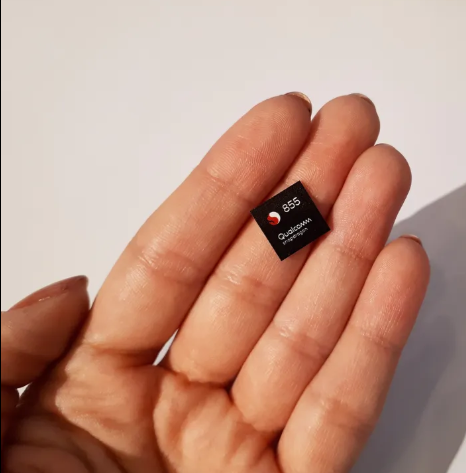
\includegraphics[width=0.8\textwidth]{images/processador_fisico.png}
        \end{column}
    \end{columns}
\end{frame}

% -------------
% Slide 5 – Número de núcleos
% -------------
\begin{frame}{Número de núcleos}
    \begin{columns}[T]
        \begin{column}{0.55\textwidth}
            Hoje é comum encontrar:
            \vspace{0.5em}
            \begin{itemize}
                \item \textbf{Dual Core} — 2 núcleos
                \item \textbf{Quad Core} — 4 núcleos
                \item \textbf{Octa Core} — 8 núcleos
                \item \textbf{Deca Core} — 10 núcleos
            \end{itemize}
        \end{column}
        \begin{column}{0.45\textwidth}
            \begin{alertblock}{Atenção}
                Nem sempre \textbf{mais núcleos} significam maior velocidade.\\[0.4em]
                O desempenho depende também da \textbf{arquitetura} e da \textbf{frequência}.
            \end{alertblock}
        \end{column}
    \end{columns}
\end{frame}

% -------------
% Slide 6 – Arquitetura CISC
% -------------
\begin{frame}{Arquitetura CISC}
    \begin{columns}[T]
        \begin{column}{0.65\textwidth}
            \begin{block}{O que é?}
                \textbf{CISC} (\textit{Complex Instruction Set Computer}) significa Computador com Conjunto de Instruções Complexas.
            \end{block}
            \vspace{0.4em}
            \textbf{Características:}
            \begin{itemize}
                \item Instruções complexas que executam várias operações.
                \item Código menor, mas execução mais lenta de cada instrução.
                \item Maior consumo de energia e dissipação de calor.
            \end{itemize}
            \vspace{0.4em}
            \begin{exampleblock}{Onde é usado?}
                Computadores de mesa e servidores (Intel x86/AMD).
            \end{exampleblock}
        \end{column}
        \begin{column}{0.35\textwidth}
            \centering
            \textbf{Fluxo CISC}
            \vspace{0.5em}
            
            \begin{tikzpicture}[
                node distance=0.5cm,
                box/.style={draw, rounded corners, fill=meuazul!15, text width=3cm, align=center, font=\footnotesize, minimum height=0.6cm},
                arrow/.style={-Stealth, thick, color=meuazul}
            ]
                \node[box] (inst) {Instrução Complexa};
                \node[box] (micro) [below=of inst] {Microcódigo (ROM)};
                \node[box] (ctrl) [below=of micro] {Unid. de Controle};
                \node[box] (exec) [below=of ctrl] {Execução (Vários ciclos)};
                
                \draw[arrow] (inst) -- (micro);
                \draw[arrow] (micro) -- (ctrl);
                \draw[arrow] (ctrl) -- (exec);
            \end{tikzpicture}
        \end{column}
    \end{columns}
\end{frame}

% -------------
% Slide 7 – Arquitetura RISC
% -------------
\begin{frame}{Arquitetura RISC}
    \begin{columns}[T]
        \begin{column}{0.65\textwidth}
            \begin{block}{O que é?}
                \textbf{RISC} (\textit{Reduced Instruction Set Computer}) significa Computador com Conjunto de Instruções Reduzidas.
            \end{block}
            \vspace{0.4em}
            \textbf{Características:}
            \begin{itemize}
                \item Instruções simples, executadas em 1 ciclo de clock.
                \item Código maior, execução extremamente rápida.
                \item Baixo consumo de energia e aquecimento.
            \end{itemize}
            \vspace{0.4em}
            \begin{exampleblock}{Onde é usado?}
                Smartphones, IoT e novos notebooks (ARM, Apple Silicon).
            \end{exampleblock}
        \end{column}
        \begin{column}{0.35\textwidth}
            \centering
            \textbf{Fluxo RISC}
            \vspace{0.5em}
            
            \begin{tikzpicture}[
                node distance=0.5cm,
                box/.style={draw, rounded corners, fill=meuvermelhoescuro!15, text width=3cm, align=center, font=\footnotesize, minimum height=0.6cm},
                arrow/.style={-Stealth, thick, color=meuvermelhoescuro}
            ]
                \node[box] (inst) {Instrução Simples};
                \node[box] (ctrl) [below=of inst] {Unid. de Controle (Hardware Direto)};
                \node[box] (exec) [below=of ctrl] {Execução (1 ciclo)};
                
                \draw[arrow] (inst) -- (ctrl);
                \draw[arrow] (ctrl) -- (exec);
            \end{tikzpicture}
        \end{column}
    \end{columns}
\end{frame}

% -------------
% Slide 8 – CISC \texttimes{} RISC
% -------------
\begin{frame}{CISC \texttimes{} RISC}
    \begin{center}
        \begin{tabular}{lll}
            \toprule
            \textbf{Característica} & \textbf{CISC} & \textbf{RISC} \\
            \midrule
            \textbf{Foco} & Hardware (instruções complexas) & Software (instruções simples) \\
            \textbf{Ciclos por instrução} & Múltiplos ciclos & Um ciclo de clock (na maioria) \\
            \textbf{Tamanho do código} & Menor & Maior \\
            \textbf{Consumo de energia} & Alto (gera mais calor) & Baixo (alta eficiência térmica) \\
            \textbf{Exemplos de uso} & PCs e Servidores (x86) & Smartphones e Tablets (ARM) \\
            \bottomrule
        \end{tabular}
    \end{center}
\end{frame}



% -------------
% Slide 10 – Arquitetura ARM
% -------------
\begin{frame}{Arquitetura ARM}
    \begin{columns}[T]
        \begin{column}{0.55\textwidth}
            \begin{block}{Por que ARM?}
                Smartphones demandam \textbf{alto desempenho} e \textbf{baixo consumo} de energia.\\[0.4em]
                Com raras exceções, os processadores de celulares são \textbf{ARM} — arquitetura \textbf{RISC} (\textit{Reduced Instruction Set Computer}).
            \end{block}
            \vspace{0.4em}
            \begin{exampleblock}{ARM Holdings}
                Empresa britânica que \textbf{desenvolve} a arquitetura, mas \textbf{não fabrica} o processador — ela \textbf{licencia} o design para outras empresas.
            \end{exampleblock}
        \end{column}
        \begin{column}{0.45\textwidth}
            \textbf{Características RISC:}
            \begin{itemize}
                \item Instruções simples e rápidas
                \item Baixo consumo energético
                \item Alta eficiência térmica
                \item Ideal para dispositivos móveis
            \end{itemize}
            \vspace{0.4em}
            \begin{alertblock}{Linha de destaque}
                A família \textbf{Cortex} é utilizada em larga escala nos smartphones de última geração.
            \end{alertblock}
        \end{column}
    \end{columns}
\end{frame}

% -------------
% Slide 7 – Famílias ARM (Tabela)
% -------------
\begin{frame}{Famílias, Arquiteturas e Núcleos ARM}
    \begin{center}
        {\footnotesize
        \begin{tabular}{lll}
            \toprule
            \textbf{Família} & \textbf{Arquitetura} & \textbf{Núcleos principais} \\
            \midrule
            ARM9TDMI  & ARMv4T    & ARM9TDMI, ARM920T, ARM922T, ARM940T \\
            \midrule
            \multirow{2}{*}{ARM9E}
                      & ARMv5TE   & ARM946E-S, ARM966E-S, ARM968E-S \\
                      & ARMv5TEJ  & ARM926EJ-S, ARM996HS \\
            \midrule
            \multirow{2}{*}{ARM10E}
                      & ARMv5TE   & ARM1020E, ARM1022E \\
                      & ARMv5TEJ  & ARM1026EJ-S \\
            \midrule
            \multirow{4}{*}{ARM11}
                      & ARMv6     & ARM1136J(F)-S \\
                      & ARMv6T2   & ARM1156T2(F)-S \\
                      & ARMv6KZ   & ARM1176JZ(F)-S \\
                      & ARMv6K    & ARM11 MPCore \\
            \midrule
            \multirow{4}{*}{\textbf{Cortex-A}}
                      & ARMv7-A   & Cortex-A5, A8, A9, A9 MPCore \\
                      & ARMv7-R   & Cortex-R4(F) \\
                      & ARMv7-M   & Cortex-M3 \\
                      & ARMv6-M   & Cortex-M0, Cortex-M1 \\
            \bottomrule
        \end{tabular}
        }
    \end{center}
    \vspace{-0.3em}
    {\tiny Fonte: ARM Holdings.}
\end{frame}
\begin{frame}{Cortex-A — A Família dos Celulares}
    \begin{center}
        \includegraphics[width=0.5\textwidth]{"images/processador cortex.png"}
    \end{center}
\end{frame}
% -------------
% Slide – Arquitetura Clássica de Computador 8 bits
% -------------
\begin{frame}{Arquitetura Clássica de um Computador de 8 bits}
\begin{center}
\resizebox{0.92\textwidth}{!}{
\begin{tikzpicture}[
    font=\small,
    box/.style={draw, rounded corners=2pt, minimum width=2cm, minimum height=0.7cm, align=center, fill=white},
    cpubox/.style={draw, thick, rounded corners=4pt, fill=meuazul!8},
    bus/.style={draw, fill=gray!20, minimum height=0.35cm},
    barr/.style={-Stealth, thick},
    dbl/.style={Stealth-Stealth, thick},
]

% ── CPU (grande retângulo) ──────────────────────────
\node[cpubox, minimum width=9cm, minimum height=5.2cm] (cpu) at (0,0) {};
\node[above, font=\bfseries\small] at (cpu.north) {CPU};

% Registradores
\node[box, fill=orange!15, minimum width=1.5cm, minimum height=0.6cm] (acc) at (-3.2, 1.4) {ACC};
\node[box, fill=orange!15, minimum width=1.5cm, minimum height=0.6cm] (pc)  at (-1.6, 1.4) {PC};
\node[box, fill=orange!15, minimum width=1.5cm, minimum height=0.6cm] (ir)  at (0,    1.4) {IR};
\node[box, fill=orange!15, minimum width=1.5cm, minimum height=0.6cm] (sp)  at (1.6,  1.4) {SP};
\node[box, fill=orange!15, minimum width=1.5cm, minimum height=0.6cm] (mar) at (3.2,  1.4) {MAR};
\node[font=\tiny, above=0.02cm of acc] {Acum.};
\node[font=\tiny, above=0.02cm of pc]  {Prog. Counter};
\node[font=\tiny, above=0.02cm of ir]  {Instr. Reg.};
\node[font=\tiny, above=0.02cm of sp]  {Stack Ptr};
\node[font=\tiny, above=0.02cm of mar] {Mem. Addr.};

% Barramento interno
\draw[gray!60, very thick] (-4, 0.7) -- (4, 0.7) node[right, font=\tiny, color=gray] {Barramento Interno (8 bits)};

% ULA
\node[box, fill=meuvermelhoescuro!20, minimum width=2.8cm, minimum height=1.2cm] (ula) at (-1.5,-0.5) {\textbf{ULA 8 bits}\\{\tiny +, -, AND, OR, NOT}};

% UC
\node[box, fill=meuverde!15, minimum width=2.8cm, minimum height=1.2cm] (uc) at (2,-0.5) {\textbf{Unidade de Controle}\\{\tiny Decodificador de Instr.}};

% Buffer E/S e Endereços
\node[box, fill=gray!15, minimum width=2cm, minimum height=0.6cm] (bufe) at (-3,-1.9) {\tiny Buffer Dados};
\node[box, fill=gray!15, minimum width=2cm, minimum height=0.6cm] (bufa) at (0.5,-1.9) {\tiny Buffer Endereços};

% Setas internas
\draw[dbl, color=meuazul] (acc.south) -- (acc.south |- 0,0.7);
\draw[dbl, color=meuazul] (ula.north) -- (0.7,0.7);
\draw[-Stealth, color=meuverde] (ir.south) -- (uc.north |- 0,0.7);
\draw[-Stealth, color=meuverde] (uc.south) -- (ula.east |- uc.south);
\draw[dbl, color=gray]  (ula.south) -- (-1.5,-1.9);
\draw[dbl, color=gray]  (uc.south)  -- (2,-1.9);

% ── Barramentos externos (fora da CPU) ─────────────
\node[bus, minimum width=11cm, minimum height=0.45cm, fill=meuazul!25]    (bdata) at (0,-3.0) {};
\node[bus, minimum width=11cm, minimum height=0.45cm, fill=orange!25]     (baddr) at (0,-3.6) {};
\node[bus, minimum width=11cm, minimum height=0.45cm, fill=meuverde!25]   (bctrl) at (0,-4.2) {};
\node[font=\tiny\bfseries, left=0.1cm of bdata] {Dados (8b)};
\node[font=\tiny\bfseries, left=0.1cm of baddr] {Endereços (16b)};
\node[font=\tiny\bfseries, left=0.1cm of bctrl] {Controle};

% Conexão CPU → barramentos
\draw[dbl, thick, color=meuazul]   (bufe.south) -- (-3,-3.0);
\draw[dbl, thick, color=orange]    (bufa.south) -- (0.5,-3.6);
\draw[-Stealth, thick, color=meuverde] (uc.south) -- (2,-4.2);

% ── RAM e ROM ──────────────────────────────────────
\node[box, fill=cyan!10, minimum width=2.2cm, minimum height=1.1cm] (ram) at (-4.2,-5.5) {\textbf{RAM}\\{\tiny Dados temporários}};
\node[box, fill=yellow!15, minimum width=2.2cm, minimum height=1.1cm] (rom) at (-1.5,-5.5) {\textbf{ROM}\\{\tiny Firmware / Boot}};

% ── E/S ───────────────────────────────────────────
\node[box, fill=purple!10, minimum width=2.2cm, minimum height=1.1cm] (io) at (2,-5.5) {\textbf{E/S}\\{\tiny Teclado, Display}};
\node[box, fill=purple!10, minimum width=2.2cm, minimum height=1.1cm] (io2) at (4.5,-5.5) {\textbf{E/S}\\{\tiny Sensores, SPI, I2C}};

% Conexões Barramentos → periféricos
\draw[dbl] (-4.2,-4.5) -- (ram.north);
\draw[dbl] (-1.5,-4.5) -- (rom.north);
\draw[dbl] (2,-4.5)    -- (io.north);
\draw[dbl] (4.5,-4.5)  -- (io2.north);

\end{tikzpicture}
}
\end{center}
\end{frame}

% -------------
% Slide 8 – Famílias Cortex por Aplicação
% -------------
\begin{frame}[allowframebreaks]{Famílias Cortex — Aplicações}
    \begin{center}
        {\small
        \begin{tabular}{lp{4cm}p{4.5cm}}
            \toprule
            \textbf{Família} & \textbf{Aplicação} & \textbf{Exemplos} \\
            \midrule
            \textbf{Cortex-A} & SO completos & Smartphones, tablets, Raspberry Pi \\
            \midrule
            \textbf{Cortex-R} & Sistemas de tempo real & HDs, SSDs, automóveis \\
            \midrule
            \textbf{Cortex-M} & Microcontroladores & Arduino Portenta, STM32 \\
            \midrule
            \textbf{Neoverse}  & Servidores e Cloud & AWS Graviton, NVIDIA Grace \\
            \midrule
            \textbf{SecurCore} & Segurança & Cartões bancários, SIM cards \\
            \bottomrule
        \end{tabular}
        }
    \end{center}
    
    \vspace{0.2em}
    \begin{center}
        \resizebox{0.85\textwidth}{!}{
        \begin{tikzpicture}[
            node distance=1.5cm,
            box/.style={draw, rounded corners, text width=2.8cm, align=center, font=\footnotesize, minimum height=1.2cm},
            cortexm/.style={box, fill=meuverde!20, draw=meuverde},
            cortexr/.style={box, fill=orange!20, draw=orange},
            cortexa/.style={box, fill=meuazul!20, draw=meuazul},
            neoverse/.style={box, fill=purple!20, draw=purple},
            securcore/.style={box, fill=yellow!50, draw=yellow!80!black}
        ]
            % Nodes
            \node[cortexm] (m) {\textbf{Cortex-M}\\Baixo consumo, IoT};
            \node[cortexr, right=of m] (r) {\textbf{Cortex-R}\\Crítico, Tempo Real};
            \node[cortexa, right=of r] (a) {\textbf{Cortex-A}\\Alto Desempenho};
            
            \node[neoverse, above=of a, yshift=-0.5cm] (neo) {\textbf{Neoverse}\\Data Center};
            \node[securcore, below=of m, yshift=0.5cm] (sec) {\textbf{SecurCore}\\Criptografia forte};
            
            % Arrows
            \draw[-Stealth, thick, color=gray] (m) -- (r) node[midway, above, font=\tiny, color=black] {+ Complexidade};
            \draw[-Stealth, thick, color=gray] (r) -- (a) node[midway, above, font=\tiny, color=black] {+ Desempenho};
            \draw[-Stealth, thick, color=gray, dashed] (a) -- (neo) node[midway, right, font=\tiny, color=black] {Escala Nuvem};
        \end{tikzpicture}
        }
    \end{center}

    \framebreak

    % Slide III
    \begin{columns}[T]
        \begin{column}{0.6\textwidth}
            \scriptsize
            \textbf{1. Núcleos de Processamento (Cortex-A9 CPU Cores)}
            \begin{itemize}
                \item \textbf{Cortex-A9 CPU:} Núcleo principal de processamento de instruções.
                \item \textbf{FPU / NEON:} Ponto flutuante e processamento vetorial SIMD (multimídia e matemática).
                \item \textbf{PTM I/F:} Depuração e rastreamento em tempo real.
                \item \textbf{I-Cache \& D-Cache:} Memórias cache L1 — I-Cache (instruções) e D-Cache (dados).
            \end{itemize}

            \textbf{2. Coerência de Cache e Interrupções}
            \begin{itemize}
                \item \textbf{SCU:} Consistência das caches L1 entre todos os núcleos.
                \item \textbf{Cache-2-Cache:} Transfere dados diretamente entre caches.
                \item \textbf{Snoop Filtering:} Filtra checagens desnecessárias.
                \item \textbf{GIC:} Roteia interrupções entre os núcleos.
                \item \textbf{ACP:} Aceleradores externos (GPU/DMA) com coerência.
            \end{itemize}
        \end{column}
        \begin{column}{0.4\textwidth}
            \centering
            \includegraphics[width=0.95\textwidth]{"images/processador cortex.png"}
        \end{column}
    \end{columns}

    \framebreak

    % Slide IV / V
    \begin{columns}[T]
        \begin{column}{0.6\textwidth}
            
            \textbf{3. Interfaces de E/S e Barramento}
            \begin{itemize}
                \item \textbf{Advanced Bus I/F:} Comunicação com a RAM e periféricos.
                \item \textbf{AMBA 3 (64-bit):} Barramento principal (AXI) para alta largura de banda.
                \item \textbf{Interface 2 (Opcional):} Balanceamento de carga ou roteamento específico.
            \end{itemize}

            \vspace{0.8em}
            \textbf{4. Depuração e Monitoramento}
            \begin{itemize}
                \item \textbf{ARM CoreSight™:} Infraestrutura global para depuração, teste e rastreamento em múltiplos núcleos simultaneamente.
            \end{itemize}
        \end{column}
        \begin{column}{0.4\textwidth}
            \centering
            \includegraphics[width=0.95\textwidth]{"images/processador cortex.png"}
        \end{column}
    \end{columns}
\end{frame}

% -------------
% Slide - Contextualização Arquitetura Clássica
% -------------
\begin{frame}{Contextualização: Arquitetura Clássica (Von Neumann)}
    \begin{columns}[T]
        \begin{column}{0.3\textwidth}
            \centering
            \textbf{Modelo Clássico}
            \vspace{0.8em}
            
            \resizebox{\linewidth}{!}{
            \begin{tikzpicture}[
                node distance=0.8cm,
                box/.style={draw, rounded corners, fill=meuazul!15, text width=2.8cm, align=center, font=\footnotesize, minimum height=0.6cm},
                arrow/.style={Stealth-Stealth, thick, color=meuazul},
                singlearrow/.style={-Stealth, thick, color=meuazul}
            ]
                % Componentes
                \node[box] (cpu) {\textbf{CPU}\\ULA, Unid. Controle,\\Registradores};
                \node[box] (mem) [below=of cpu] {\textbf{Memória Principal}\\(Instruções e Dados)};
                \node[box] (io) [below=of mem] {\textbf{Dispositivos de E/S}};
                
                % Barramento do Sistema
                \node[draw, fill=meucinza!20, minimum height=5cm, minimum width=0.5cm, right=0.8cm of mem, label=above:{\scriptsize \shortstack{Barramento\\do Sistema}}] (bus) {};
                
                % Conexões
                \draw[arrow] (cpu.east) -- (cpu.east -| bus.west);
                \draw[arrow] (mem.east) -- (mem.east -| bus.west);
                \draw[arrow] (io.east)  -- (io.east -| bus.west);
            \end{tikzpicture}
            }
        \end{column}
        \begin{column}{0.7\textwidth}
            \begin{block}{Paralelo com o Cortex-A9 (Moderna)}
                A arquitetura clássica evoluiu para lidar com múltiplos núcleos e alta demanda:
                \vspace{0.5em}
                \begin{itemize}
                    \item \textbf{CPU Clássica} $\rightarrow$ \textbf{Núcleos Cortex}: Agora cada núcleo possui sua própria ULA, NEON (FPU) e memórias \textbf{Cache L1} embutidas.
                    \item \textbf{Barramento do Sistema} $\rightarrow$ \textbf{Interface AMBA / SCU}: O gargalo do barramento clássico exigiu a criação do \textit{Snoop Control Unit} para manter a coerência das caches sem sobrecarregar a RAM.
                    \item \textbf{E/S e Interrupções} $\rightarrow$ \textbf{GIC e ACP}: Controladores dedicados de interrupção agora roteiam eventos dinamicamente para os núcleos livres.
                \end{itemize}
            \end{block}
        \end{column}
    \end{columns}
\end{frame}


% -------------
% Slide 9 – Cortex-A: a família dos celulares
% -------------
\begin{frame}{Cortex-A — A Família dos Celulares}
    \begin{columns}[T]
        \begin{column}{0.5\textwidth}
            \begin{block}{Por que Cortex-A?}
                É a família utilizada em \textbf{celulares e tablets}.\\[0.4em]
                \textbf{Características:}
                \begin{itemize}
                    \item Alto desempenho
                    \item Suporte a memória virtual (MMU)
                    \item Linux, Android e iOS
                    \item Suporte a \textbf{multicore}
                \end{itemize}
            \end{block}
        \end{column}
        \begin{column}{0.5\textwidth}
            \textbf{Exemplos de núcleos:}
            \vspace{0.3em}

            {\footnotesize
            \begin{tabular}{ll}
                Cortex-A5   & Cortex-A53 \\
                Cortex-A7   & Cortex-A55 \\
                Cortex-A8   & Cortex-A57 \\
                Cortex-A9   & Cortex-A72 \\
                Cortex-A15  & Cortex-A73 \\
                Cortex-A17  & Cortex-A75 \\
                Cortex-A35  & Cortex-A76 \\
                Cortex-A77  & Cortex-A78 \\
                Cortex-X1   & Cortex-X2  \\
                Cortex-X3   & Cortex-X4  \\
                \multicolumn{2}{l}{Cortex-X925} \\
            \end{tabular}
            }
            \vspace{0.5em}
            
        \end{column}
    \end{columns}
\end{frame}

% =============================================================
\section{GPU, Memória e Armazenamento}
% =============================================================

% -------------
% Slide 8 – GPU (renumerado)
% -------------
\begin{frame}{GPU — Graphics Processing Unit}
    \begin{columns}[T]
        \begin{column}{0.55\textwidth}
            \begin{block}{Responsável por:}
                \begin{itemize}
                    \item Jogos
                    \item Animações
                    \item Vídeos
                    \item Inteligência artificial
                    \item Realidade aumentada
                \end{itemize}
            \end{block}
        \end{column}
        \begin{column}{0.45\textwidth}
            \begin{exampleblock}{Exemplo}
                Jogos como \textbf{PUBG} e \textbf{Call of Duty} usam intensamente a GPU.
            \end{exampleblock}
        \end{column}
    \end{columns}
\end{frame}

% -------------
% Slide 7 – Memória RAM
% -------------
\begin{frame}{Memória RAM}
    \begin{columns}[T]
        \begin{column}{0.5\textwidth}
            \begin{block}{O que é?}
                A RAM armazena \textbf{temporariamente} os dados dos aplicativos em execução.\\[0.4em]
                Quanto maior a RAM:
                \begin{itemize}
                    \item mais aplicativos podem permanecer abertos;
                    \item menor necessidade de recarregar aplicativos.
                \end{itemize}
            \end{block}
        \end{column}
        \begin{column}{0.5\textwidth}
            \textbf{Referência de uso:}
            \vspace{0.4em}

            \begin{tabular}{ll}
                \toprule
                \textbf{RAM} & \textbf{Uso típico} \\
                \midrule
                4 GB  & Navegação básica \\
                8 GB  & Multitarefa \\
                12 GB+ & Jogos e edição de vídeo \\
                \bottomrule
            \end{tabular}
            \vspace{1em}
            
            \centering
            \includegraphics[width=0.6\textwidth]{"images/ram.png"}
        \end{column}
    \end{columns}
\end{frame}

% -------------
% Slide 8 – Armazenamento
% -------------
\begin{frame}{Armazenamento}
    \begin{columns}[T]
        \begin{column}{0.5\textwidth}
            \textbf{Onde ficam gravados:}
            \begin{itemize}
                \item Aplicativos
                \item Fotos
                \item Vídeos
                \item Documentos
            \end{itemize}
            \vspace{0.5em}
            \textbf{Capacidades comuns:}\\
            64 GB \quad 128 GB \quad 256 GB \quad 512 GB \quad 1 TB
        \end{column}
        \begin{column}{0.5\textwidth}
            \begin{alertblock}{Diferença fundamental}
                \textbf{RAM} → memória temporária\\[0.3em]
                \textbf{Armazenamento} → memória permanente
            \end{alertblock}
            \vspace{1em}
            
            \centering
            \includegraphics[width=0.7\textwidth]{"images/flash.png"}
        \end{column}
    \end{columns}
\end{frame}

% -------------
% Slide 8.5 – Câmeras
% -------------
\begin{frame}{Câmeras}
    \begin{columns}[T]
        \begin{column}{0.5\textwidth}
            \textbf{Evolução constante:}
            \begin{itemize}
                \item De lentes simples a conjuntos triplos ou quádruplos.
                \item Processamento de imagem por IA (fotografia computacional).
                \item Captura de vídeo em 4K e 8K.
            \end{itemize}
        \end{column}
        \begin{column}{0.5\textwidth}
            \centering
            \includegraphics[width=0.7\textwidth]{"images/camera.png"}
        \end{column}
    \end{columns}
\end{frame}

% =============================================================
\section{Sensores e Atuadores}
% =============================================================

% -------------
% Slide 9 – Sensores
% -------------
\begin{frame}{Sensores}
    \begin{columns}[T]
        \begin{column}{0.55\textwidth}
            \begin{block}{Um smartphone possui dezenas de sensores:}
                \begin{itemize}
                    \item GPS
                    \item Acelerômetro
                    \item Giroscópio
                    \item Bússola
                    \item Proximidade
                    \item Luminosidade
                    \item Leitor biométrico
                    \item Barômetro
                \end{itemize}
            \end{block}
        \end{column}
        \begin{column}{0.45\textwidth}
            \begin{exampleblock}{Atividade}
                Mostre exemplos de aplicativos que utilizam cada sensor.
            \end{exampleblock}
        \end{column}
    \end{columns}
\end{frame}

% -------------
% Slide 10 – Acelerômetro
% -------------
\begin{frame}{Acelerômetro}
    \begin{columns}[T]
        \begin{column}{0.5\textwidth}
            \begin{block}{O que faz?}
                Detecta \textbf{movimentos} do dispositivo.
            \end{block}
            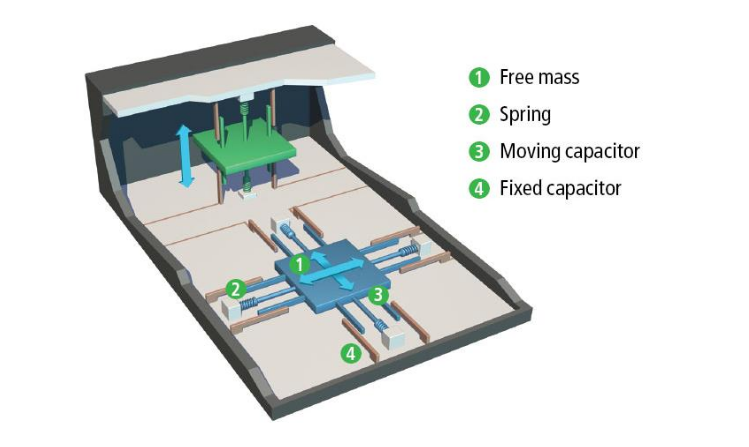
\includegraphics[height=4cm]{images/acelerometro2.png}
        \end{column}
        \begin{column}{0.5\textwidth}
            \textbf{Aplicações:}
            \begin{itemize}
                \item Girar a tela
                \item Contar passos
                \item Detectar quedas
                \item Jogos
            \end{itemize}
            \vspace{0.5em}
            \centering
            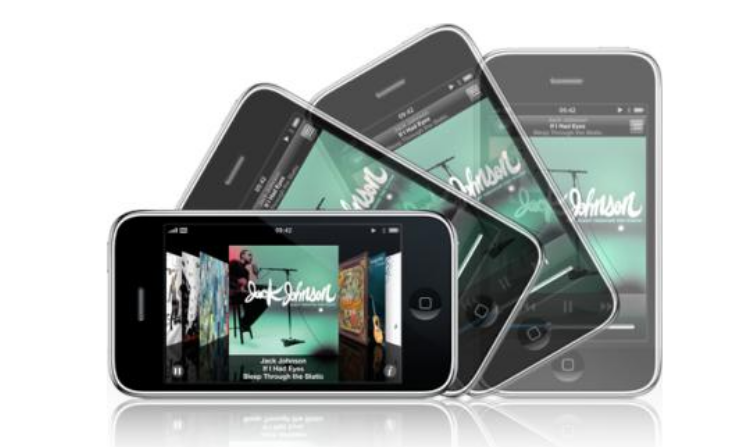
\includegraphics[height=4cm]{images/acelerometro1.png}
            \quad
        \end{column}
    \end{columns}
\end{frame}

% -------------
% Slide 11 – GPS
% -------------
\begin{frame}{GPS}
    \begin{columns}[T]
        \begin{column}{0.5\textwidth}
            \begin{block}{O que faz?}
                Determina a \textbf{localização geográfica} do dispositivo.
            \end{block}
            \includegraphics[height=4cm]{"images/gps.png"}

        \end{column}
        \begin{column}{0.5\textwidth}
            \textbf{Aplicações:}
            \begin{itemize}
                \item Uber
                \item Google Maps
                \item iFood
                \item Pokémon GO
            \end{itemize}
        \end{column}
    \end{columns}
\end{frame}

% -------------
% Slide 12 – Giroscópio
% -------------
\begin{frame}{Giroscópio}
    \begin{columns}[T]
        \begin{column}{0.5\textwidth}
            \begin{block}{O que faz?}
                Mede \textbf{rotações} do aparelho.
            \end{block}
            \includegraphics[height=3cm]{"images/giroscopio.jpg"}
        \end{column}
        \begin{column}{0.5\textwidth}
            \textbf{Muito usado em:}
            \begin{itemize}
                \item Realidade virtual
                \item Realidade aumentada
                \item Jogos
            \end{itemize}
            \vspace{0.5em}
            \centering
            \quad
            \includegraphics[height=4cm]{"images/giroscopio_posicoes.jpg"}
        \end{column}
    \end{columns}
\end{frame}

% -------------
% Slide 13 – Sensores de proximidade
% -------------
\begin{frame}{Sensores de Proximidade}
    \begin{columns}[T]
        \begin{column}{0.5\textwidth}
            \begin{block}{O que fazem?}
                Detectam \textbf{objetos próximos} ao dispositivo.
            \end{block}
            \includegraphics[height=4cm]{"images/proximidade1.png"}
        \end{column}
        \begin{column}{0.5\textwidth}
            \begin{exampleblock}{Exemplo clássico}
                Durante uma ligação, o celular \textbf{desliga a tela} quando aproximado da orelha.
            \end{exampleblock}
            \vspace{0.5em}
            \centering
            \quad
            \includegraphics[height=3cm]{"images/proximidade2.png"}
        \end{column}
    \end{columns}
\end{frame}

% -------------
% Slide 14 – Sensores de luminosidade
% -------------
\begin{frame}{Sensores de Luminosidade}
    \begin{columns}[T]
        \begin{column}{0.5\textwidth}
            \begin{block}{O que fazem?}
                Ajustam \textbf{automaticamente} o brilho da tela conforme o ambiente.
            \end{block}
        \end{column}
        \begin{column}{0.5\textwidth}
            \textbf{Benefícios:}
            \begin{itemize}
                \item Economia de bateria
                \item Conforto visual
            \end{itemize}
            \vspace{0.5em}
            \centering
            \includegraphics[width=0.85\textwidth]{"images/luminosidade.png"}
        \end{column}
    \end{columns}
\end{frame}

% -------------
% Slide – Visão Geral: Sensores do Smartphone
% -------------
\begin{frame}{Visão Geral: Sensores do Smartphone}
    \begin{columns}[T]
        \begin{column}{0.5\textwidth}
            \begin{block}{Sensores captam o ambiente}
                \begin{itemize}
                    \item \textbf{Acelerômetro:} Mede aceleração e gravidade (orientação da tela).
                    \item \textbf{Giroscópio:} Rotação 3D — VR, jogos e estabilização de câmera.
                    \item \textbf{Proximidade:} Detecta objetos perto da tela (desliga visor na ligação).
                    \item \textbf{Luz Ambiente:} Ajusta brilho da tela automaticamente.
                    \item \textbf{Magnetômetro:} Bússola digital para mapas e navegação.
                \end{itemize}
            \end{block}
        \end{column}
        \begin{column}{0.5\textwidth}
            \begin{block}{Sensores de localização e biometria}
                \begin{itemize}
                    \item \textbf{GPS:} Capta sinais de satélite para localização exata.
                    \item \textbf{Barômetro:} Mede pressão atmosférica e altitude; melhora precisão do GPS.
                    \item \textbf{Digital (Biométrico):} Leitor de impressão digital (ultrassônico, óptico ou capacitivo).
                    \item \textbf{Câmera frontal:} Reconhecimento facial 2D/3D.
                \end{itemize}
            \end{block}
        \end{column}
    \end{columns}
\end{frame}

% -------------
% Slide – Atuadores do Smartphone
% -------------
\begin{frame}{Atuadores do Smartphone}
    \begin{block}{Atuadores convertem comandos elétricos em ações físicas}
    \end{block}
    \vspace{0.4em}
    \begin{columns}[T]
        \begin{column}{0.5\textwidth}
            \begin{itemize}
                \item \textbf{Motor de Vibração (Tátil):} Converte sinais elétricos em vibrações e respostas hápticas ao digitar ou receber notificações.
                \item \textbf{Alto-falante / Fone:} Transformam sinais de áudio elétricos em ondas sonoras.
                \item \textbf{Tela (LCD/OLED):} Atuador visual — converte dados digitais em imagens coloridas e luz.
            \end{itemize}
        \end{column}
        \begin{column}{0.5\textwidth}
            \begin{itemize}
                \item \textbf{LEDs / Flash da Câmera:} Converte eletricidade em feixes de luz visíveis.
                \item \textbf{Motor de Foco (VCM/OIS):} Minúsculos motores (Voice Coil Motor) que movem as lentes para focar e estabilizar imagens.
            \end{itemize}
            \vspace{0.5em}
            \begin{exampleblock}{Sensores \texttimes{} Atuadores}
                \textbf{Sensores} captam o mundo; \textbf{Atuadores} agem sobre ele.
            \end{exampleblock}
        \end{column}
    \end{columns}
\end{frame}

% =============================================================
\section{Bateria}
% =============================================================

% -------------
% Slide 15 – Bateria
% -------------
\begin{frame}{Bateria}
    \begin{columns}[T]
        \begin{column}{0.55\textwidth}
            \begin{block}{A bateria fornece energia ao dispositivo.}
                \textbf{Características:}
                \begin{itemize}
                    \item Medida em mAh
                    \item Ciclos de carga
                    \item Carregamento rápido
                    \item Carregamento sem fio
                \end{itemize}
            \end{block}
        \end{column}
        \begin{column}{0.45\textwidth}
            \begin{alertblock}{Impacto no desenvolvimento}
                Quanto maior o consumo do aplicativo, \textbf{maior será o gasto energético}.
            \end{alertblock}
        \end{column}
    \end{columns}
\end{frame}

% -------------
% Slide 16 – O hardware influencia o desenvolvimento?
% -------------
% =============================================================
\section{Hardware e Desenvolvimento}
% =============================================================

\begin{frame}{O hardware influencia o desenvolvimento?}
    \begin{center}
        \Large\textbf{Sim.}
    \end{center}
    \vspace{0.3em}
    \begin{columns}[T]
        \begin{column}{0.33\textwidth}
            \begin{block}{App de câmera}
                \begin{itemize}
                    \item CPU
                    \item GPU
                    \item Memória
                    \item Sensores
                    \item Armazenamento
                \end{itemize}
            \end{block}
        \end{column}
        \begin{column}{0.33\textwidth}
            \begin{block}{App de navegação}
                \begin{itemize}
                    \item GPS
                    \item Internet
                    \item Bateria
                \end{itemize}
            \end{block}
        \end{column}
        \begin{column}{0.33\textwidth}
            \begin{block}{App de RA}
                \begin{itemize}
                    \item Câmera
                    \item GPU
                    \item Giroscópio
                \end{itemize}
            \end{block}
        \end{column}
    \end{columns}
\end{frame}

% =============================================================
\section{Sistemas Operacionais Móveis}
% =============================================================

% -------------
% Slide 17 – Sistemas Operacionais Móveis
% -------------
\begin{frame}{Sistemas Operacionais Móveis}
    \begin{columns}[T]
        \begin{column}{0.5\textwidth}
            \begin{block}{Os dois principais são:}
                \begin{itemize}
                    \item \textbf{Android}
                    \item \textbf{iOS}
                \end{itemize}
            \end{block}
        \end{column}
        \begin{column}{0.5\textwidth}
            \textbf{Eles controlam:}
            \begin{itemize}
                \item Hardware
                \item Memória
                \item Segurança
                \item Aplicativos
                \item Comunicação
            \end{itemize}
        \end{column}
    \end{columns}
\end{frame}

% -------------
% Slide 18 – Android
% -------------
\begin{frame}{Android}
    \begin{columns}[T]
        \begin{column}{0.55\textwidth}
            \begin{block}{Desenvolvido pelo Google}
                \textbf{Características:}
                \begin{itemize}
                    \item Código aberto (AOSP)
                    \item Utilizado por diversas fabricantes
                    \item Altamente personalizável
                    \item Maior participação no mercado mundial
                \end{itemize}
            \end{block}
        \end{column}
        \begin{column}{0.45\textwidth}
            \textbf{Fabricantes:}
            \begin{itemize}
                \item Samsung
                \item Motorola
                \item Xiaomi
                \item Realme
                \item Honor
            \end{itemize}
            \vspace{0.5em}
            \centering
            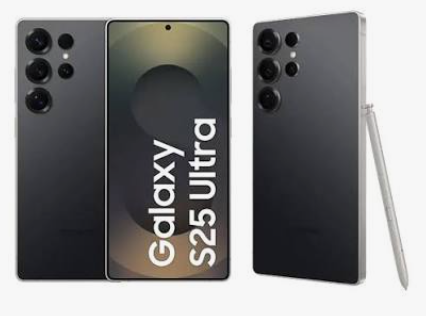
\includegraphics[width=0.4\textwidth]{images/sansung.png}
            \quad
            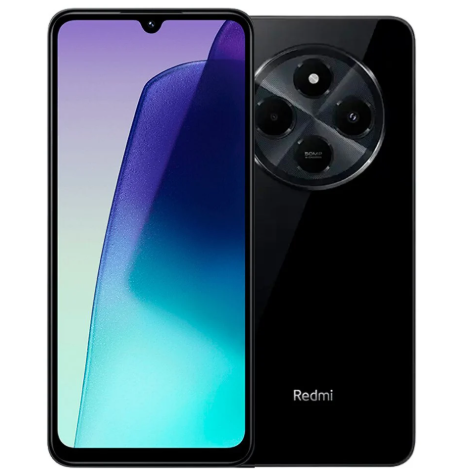
\includegraphics[width=0.4\textwidth]{images/xiaomi.png}
        \end{column}
    \end{columns}
\end{frame}

% -------------
% Slide 19 – Arquitetura Android
% -------------
\begin{frame}{Arquitetura Android}
    \begin{columns}[T]
        \begin{column}{0.45\textwidth}
            \textbf{Fluxo simplificado:}
            \vspace{0.5em}

            \begin{tikzpicture}[
                node distance=0.55cm,
                every node/.style={draw, rounded corners, fill=meuazul!15,
                    text width=3.8cm, align=center, font=\small},
                arrow/.style={-Stealth, thick, color=meuazul}
            ]
                \node (app)  {Aplicativos};
                \node (fw)   [below=of app]  {Framework Android};
                \node (art)  [below=of fw]   {Android Runtime (ART)};
                \node (lib)  [below=of art]  {Bibliotecas Nativas};
                \node (ker)  [below=of lib]  {Kernel Linux};
                \node (hw)   [below=of ker]  {Hardware};
                \draw[arrow] (app) -- (fw);
                \draw[arrow] (fw)  -- (art);
                \draw[arrow] (art) -- (lib);
                \draw[arrow] (lib) -- (ker);
                \draw[arrow] (ker) -- (hw);
            \end{tikzpicture}
        \end{column}
        \begin{column}{0.55\textwidth}
            \textbf{Cada camada:}
            \vspace{0.3em}
            \begin{description}
                \item[\textbf{Aplicativos}] Apps instalados pelo usuário.
                \item[\textbf{Framework}] Disponibiliza APIs para os apps.
                \item[\textbf{ART}] Executa os aplicativos.
                \item[\textbf{Kernel Linux}] Controla memória, processos e drivers.
                \item[\textbf{Hardware}] CPU, câmera, sensores etc.
            \end{description}
        \end{column}
    \end{columns}
\end{frame}

% -------------
% Slide 20 – iOS
% -------------
\begin{frame}{iOS}
    \begin{columns}[T]
        \begin{column}{0.55\textwidth}
            \begin{block}{Desenvolvido pela Apple}
                \textbf{Características:}
                \begin{itemize}
                    \item Sistema proprietário
                    \item Exclusivo para iPhone
                    \item Forte integração hardware-software
                    \item Atualizações simultâneas
                    \item Alto desempenho
                \end{itemize}
            \end{block}
        \end{column}
        \begin{column}{0.45\textwidth}
            \begin{alertblock}{Diferencial}
                A Apple controla \textbf{hardware e software}, garantindo maior otimização e segurança.
            \end{alertblock}
            \vspace{0.5em}
            \centering
            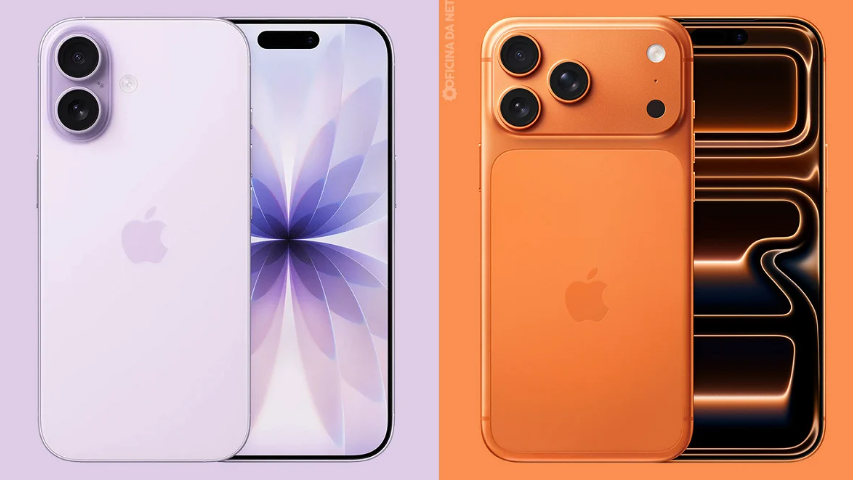
\includegraphics[width=0.6\textwidth]{images/iphone.png}
        \end{column}
    \end{columns}
\end{frame}

% -------------
% Slide 21 – Arquitetura do iOS
% -------------
\begin{frame}{Arquitetura do iOS}
    \begin{columns}[T]
        \begin{column}{0.45\textwidth}
            \textbf{Fluxo simplificado:}
            \vspace{0.5em}

            \begin{tikzpicture}[
                node distance=0.6cm,
                every node/.style={draw, rounded corners, fill=meuvermelhoescuro!15,
                    text width=3.8cm, align=center, font=\small},
                arrow/.style={-Stealth, thick, color=meuvermelhoescuro}
            ]
                \node (app)  {Aplicativos};
                \node (fw)   [below=of app]  {Frameworks};
                \node (cs)   [below=of fw]   {Core Services};
                \node (co)   [below=of cs]   {Core OS};
                \node (hw)   [below=of co]   {Hardware};
                \draw[arrow] (app) -- (fw);
                \draw[arrow] (fw)  -- (cs);
                \draw[arrow] (cs)  -- (co);
                \draw[arrow] (co)  -- (hw);
            \end{tikzpicture}
        \end{column}
        \begin{column}{0.55\textwidth}
            \begin{block}{Características da arquitetura}
                \begin{description}
                    \item[\textbf{Aplicativos}] Apps da App Store e nativos.
                    \item[\textbf{Frameworks}] UIKit, SwiftUI, CoreML etc.
                    \item[\textbf{Core Services}] Serviços fundamentais do sistema.
                    \item[\textbf{Core OS}] Kernel XNU baseado em BSD/Mach.
                    \item[\textbf{Hardware}] SoC Apple (CPU + GPU integrados).
                \end{description}
            \end{block}
        \end{column}
    \end{columns}
\end{frame}

% -------------
% Slide 22 – Android × iOS
% -------------
\begin{frame}{Android \texttimes{} iOS}
    \begin{center}
        \begin{tabular}{lll}
            \toprule
            \textbf{Característica}     & \textbf{Android}          & \textbf{iOS} \\
            \midrule
            Licença                    & Código aberto (AOSP)      & Proprietário \\
            Fabricantes                & Múltiplos                 & Apenas Apple \\
            Personalização             & Alta                      & Menor \\
            Linguagens                 & Java / Kotlin             & Swift / Objective-C \\
            Hardware                   & Diversidade               & Padronizado \\
            Loja de apps               & Google Play               & App Store \\
            \bottomrule
        \end{tabular}
    \end{center}
\end{frame}

% -------------
% Slide 23 – Como isso afeta o desenvolvedor?
% -------------
\begin{frame}{Como isso afeta o desenvolvedor?}
    \begin{columns}[T]
        \begin{column}{0.55\textwidth}
            \begin{block}{O programador deve considerar:}
                \begin{itemize}
                    \item Diferentes tamanhos de tela;
                    \item Quantidade de memória;
                    \item Desempenho do processador;
                    \item Consumo de bateria;
                    \item Disponibilidade de sensores;
                    \item Permissões do sistema.
                \end{itemize}
            \end{block}
        \end{column}
        \begin{column}{0.45\textwidth}
            \begin{alertblock}{Reflexão}
                Um app bem desenvolvido respeita as limitações do dispositivo e oferece boa experiência a todos os usuários.
            \end{alertblock}
        \end{column}
    \end{columns}
\end{frame}

% -------------
% Slide 24 – Boas práticas
% -------------
\begin{frame}{Boas Práticas no Desenvolvimento Móvel}
    \begin{columns}[T]
        \begin{column}{0.5\textwidth}
            \begin{alertblock}{Evitar:}
                \begin{itemize}
                    \item Consumo excessivo de bateria;
                    \item Uso contínuo do GPS;
                    \item Processamento pesado;
                    \item Uso desnecessário da câmera;
                    \item Excesso de memória.
                \end{itemize}
            \end{alertblock}
        \end{column}
        \begin{column}{0.5\textwidth}
            \begin{block}{Objetivo:}
                Aplicativos \textbf{rápidos} e \textbf{eficientes}.
            \end{block}
        \end{column}
    \end{columns}
\end{frame}

\end{document}
